% TIPO DE DOCUMENTO
\documentclass[12pt]{article}

% region PAQUETES QUE VAMOS A USAR
\usepackage{amsmath}
\usepackage{amssymb} 
\usepackage[utf8]{inputenc} 
\usepackage[spanish]{babel} 
\usepackage{comment}
\usepackage{graphicx}
\usepackage{wrapfig}
\usepackage{float}
\usepackage{xcolor}
\usepackage{tikz}
\usepackage{emptypage}
\usepackage{geometry}
\usepackage{amsthm}
\usepackage{url}
\usepackage[colorlinks=true,linkcolor=]{hyperref}
\usepackage[all]{xy}
\usepackage{fancyhdr}
\usepackage{pdfpages}
\usepackage{lipsum}
\usepackage{fix-cm}
\usepackage{yhmath}
\usepackage{microtype}
\usepackage{multimedia}
% endregion

\usetikzlibrary{calc, arrows.meta, babel}

% --- CONFIGURACIÓN DE ESPACIADO ENTRE PÁRRAFOS ---
\setlength{\parskip}{2mm}

% region ABREVIATURAS
\newcommand{\N}{\mathbb{N}}
\newcommand{\R}{\mathbb{R}}
\newcommand{\F}{\mathcal{F}}
\newcommand{\A}{\mathcal{A}}
% endregion

% region DEFINIMOS LOS ENTORNOS
\theoremstyle{definition}
\newtheorem{teorema}{Teorema}[section] % Teorema es el contador principal que se reinicia por sección

% Los demás comparten el contador [teorema] para seguir la misma numeración correlativa
\newtheorem{definicion}[teorema]{\textbf{Definición}}
\newtheorem{nota}[teorema]{Nota}
\newtheorem{propiedad}[teorema]{Propiedades}
\newtheorem{definiciones}[teorema]{Definiciones}

\newtheorem*{nota*}{Nota}
\newtheorem*{teorema*}{Teorema}
% endregion

% --- MODIFICACIÓN DEL TÍTULO DEL ÍNDICE ---
\renewcommand{\contentsname}{Índice General}

% MÁRGENES DESEADOS
\geometry{a4paper,left=2cm,right=2cm,top=2cm,bottom=2cm}

% --- ARREGLO PARA FANCYHDR ---
\setlength{\headheight}{16pt} 

% INDENTACION
\setlength{\parindent}{0pt} 

%%%%%%%%%%%%%%%%%%%%%%%%%%%%%%%%%%%%%%%%%%%%%%%%%%%%%%%
%%%%%%%% variables de la cabecera %%%%%%%%%%%%%%%%%%%%%
%%%%%%%%%%%%%%%%%%%%%%%%%%%%%%%%%%%%%%%%%%%%%%%%%%%%%%%

\newcommand{\tituloacademico}{Grado en Matemáticas}

\newcommand{\documento}{PRINCIPIO DE INCERTIDUMBRE DE HEISENBERG}

\newcommand{\fechatrabajo}{Noviembre 2026}
\newcommand{\autor}{Álvaro Rivero Horrillo}

% -------------------------------------------------------------------------------------------------------------------------------------------%

\begin{document}

\begin{titlepage}
% Lado izqdo. de la p\'agina
\begin{minipage}{0.20\textwidth}
\begin{flushleft}
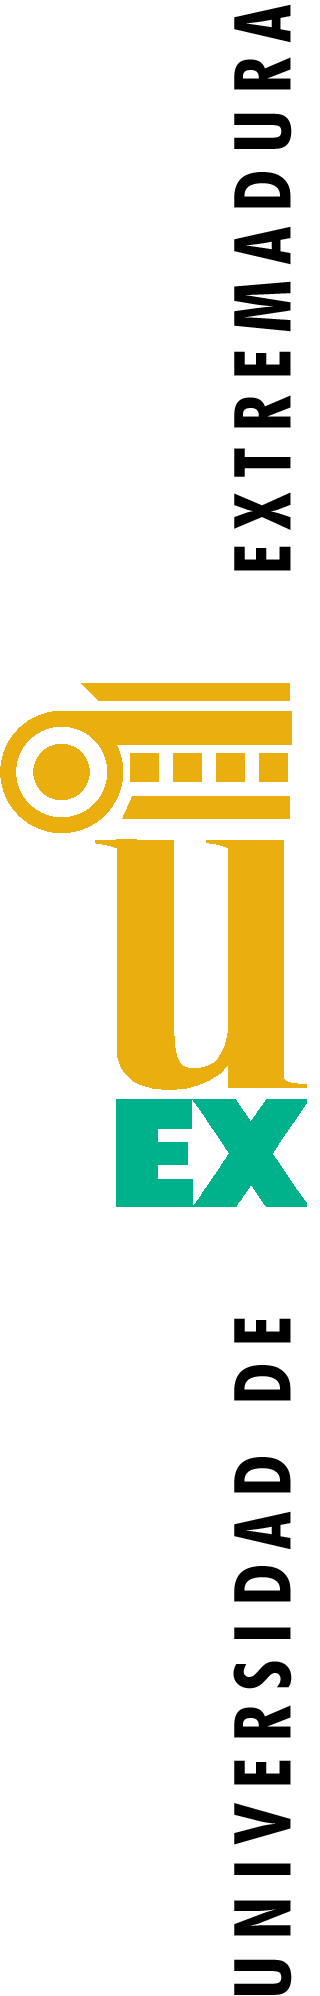
\includegraphics[scale=0.3, width=3cm]{./logos/marca_UEx_4_color.png}
\end{flushleft}
\end{minipage}
% Lado derecho de la p\'agina
\begin{minipage}{0.78\textwidth}

\vspace{3cm}

\centering
    \textsc{\LARGE Facultad de Ciencias}\\[1cm]
    \textsc{\Large \tituloacademico}\\[1cm]
    \textsc{\large AMPLIACIÓN DE VARIABLE COMPLEJA}\\[4cm]

\centering
    
    \textsc{\large \documento}\\[3cm]

\flushright
\textsc{\normalsize \autor}\\

\vspace{5mm}

\textsc{\normalsize \fechatrabajo}\\
\end{minipage}

\end{titlepage}

\tableofcontents

\newpage 

\pagestyle{plain} 

\section{Introducción}

\newpage

\section{Propiedades Básicas de las Series de Fourier}

En esta sección, comenzaremos nuestro estudio de las series de Fourier. Prepararemos el terreno introducciendo los principales conceptos que usaremos y formularemos problemas que iremos resolviendo a la vez.

Pero antes, daremos una breve descripción de los tipos de funciones sobre las que debemos preocuparnos. Puesto que podemos usar la siguiente definición provisional de coeficientes de Fourier de una función $f$:

\begin{equation*}
    a_n = \frac{1}{L} \int_{0}^{L} f(x)e^{-2\pi inx/L} \,dx; \hspace{5mm} \text{para \(n \in \mathbb{Z}\)},
\end{equation*}

donde \(f\) es una función compleja en \([0,L]\). De aquí en adelante asumiremos que todas las funciones que tratemos, son al menos Riemann integrables. Principalmente trataremos funciones de los siguientes tipos:

\begin{enumerate}
    \item \textbf{Funciones continuas en todo punto (a):} Son funciones complejas \(f\) que son continuas en todo punto del intervalo \([0,L]\).
    \item \textbf{Funciones continuas a trozos (b):} Estas serán funciones acotadas en \([0,L]\) que tienen un número finito de discontinuidades.
\end{enumerate}

\begin{figure}[ht]
    \centering
    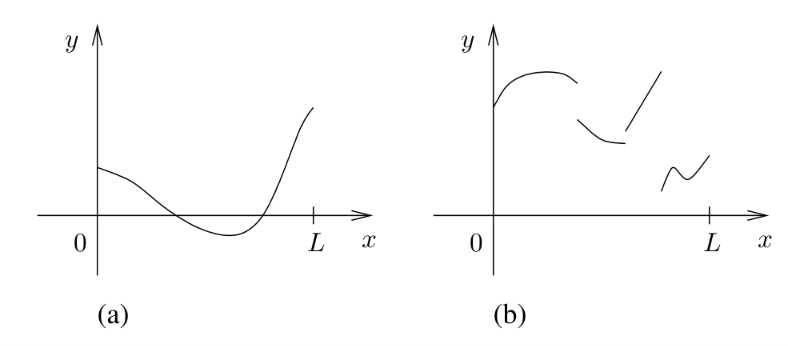
\includegraphics[width=0.8\textwidth]{graficas.png}
    \caption{Funciones en \([0,L]\): continua en todo punto y a trozos}
\end{figure}

    \subsection{Principales definiciones y ejemplos}

    \subsection{Convolución}

    \subsection{Buenos núcleos}

\newpage

\section{Convergencia de las Series de Fourier}

    \subsection{Convergencia en media cuadrática de las Series de Fourier}
        
        \subsubsection{Espacion vectoriales y productos escalares}

        \subsubsection{Prueba del teorema de convergencia en media cuadrática}

\newpage

\section{La transformada de Fourier en \texorpdfstring{\(\mathbb{R}\)}{R}}

    \subsection{Teoría elemental de la transformada de Fourier}
        
        \subsubsection{Integración de funciones en la recta real}

        \subsubsection{Definición de la transformada de Fourier}

        \subsubsection{Espacio de Schwartz}

        \subsubsection{La transformada de Fourier en \texorpdfstring{\(\mathcal{S}\)}{S}}

        \subsubsection{Inversión de Fourier}

        \subsubsection{Fórmula de Plancherel}

    \subsection{Principio de Incertidumbre de Heisenberg}

\newpage

% --- CONFIGURACIÓN DE LA BIBLIOGRAFÍA EN EL ÍNDICE ---
\clearpage
\phantomsection
\addcontentsline{toc}{section}{Bibliografía}

\nocite{*}
\bibliographystyle{plain} 
\bibliography{bibliografia}

\end{document}